\subsubsection{Imprinted Nanoparticles}
\index{Fernandez-Lahore, Marcelo}

The work of Professor Fernandez-Lahore's group at IUB has the main
goal of the meta-integration between the various bioproduct
purification strategies that have been described
 previously in an isolate manner. The prefix meta- is thus
 ''used with the name of a discipline to designate a new but
  related discipline designed to deal critically with the original
  one''  (Webster Dictionary). Up to now, no general rules exist on how to
   combine in the more efficient way process and material technology,
combinatorial techniques, and genetic engineering tools. We are
exploring this situation utilising a number of relevant industrial
(bio) products. From the knowledge generated within the frame of
our project(s) it is expected that general recommendations to
guide industrialists will emerge. Clearly, this will translate in
facilitated bioprocessing.



\paragraph{Highlights}
%
The modern Life science and Bio-Chemical industry heavily depends
on the availability of efficient processes, which should be able
to generate competitive products in terms of quality and cost. A
critical assessment of current bioprocess technology will reveal
that important bottlenecks still exist at the product recovery and
purification level. One possible route for downstream process
intensification is via direct product separation utilising novel
adsorbents materials with high affinity, competitive capacity,
reversibly interaction, and enough robustness for process
applications.

This project proposes the utilisation of molecularly imprinted
colloidal spheres produce via gamma radiation polymerisation
methods. This technique can produce imprinted polymers with
increased capacity and quality as compared to the thermal and
photochemical initiation processes. Thus, radiation-induced
sub-micrometer beads can behave as nano-to-micro reactors for
imprinted polymers therefore leading to the creation of artificial
receptors for valuable biochemical products. Carminic acid, a
natural food colorant, will be employed as a model template
molecule.

Colloidal particles with artificial recognition properties will be
subsequently integrated into downstream processing systems,
particularly for natural product recovery e.g. by embedding into
macro-porous 3D structures. The mass transfer properties and the
sorption performance of the hybrid system will be quantitatively
described. Application to real process feedstock could be
advantageous due to low operating pressures and biomass tolerance.
Alternatively, the utilisation of imprinted colloid particles as
collectors for foam flotation and their application for selective
recovery in aqueous two-phase systems will also be tested.

The proposed approach creates the opportunity to for nano-scale
engineering in order to enhance industrial process performance, as
applied to natural or bio-synthetic product recovery. These
developments are expected to positively impact in the
pharmaceutical, food, and chemical industry.




\begin{figure}[ht]
  \begin{center}
   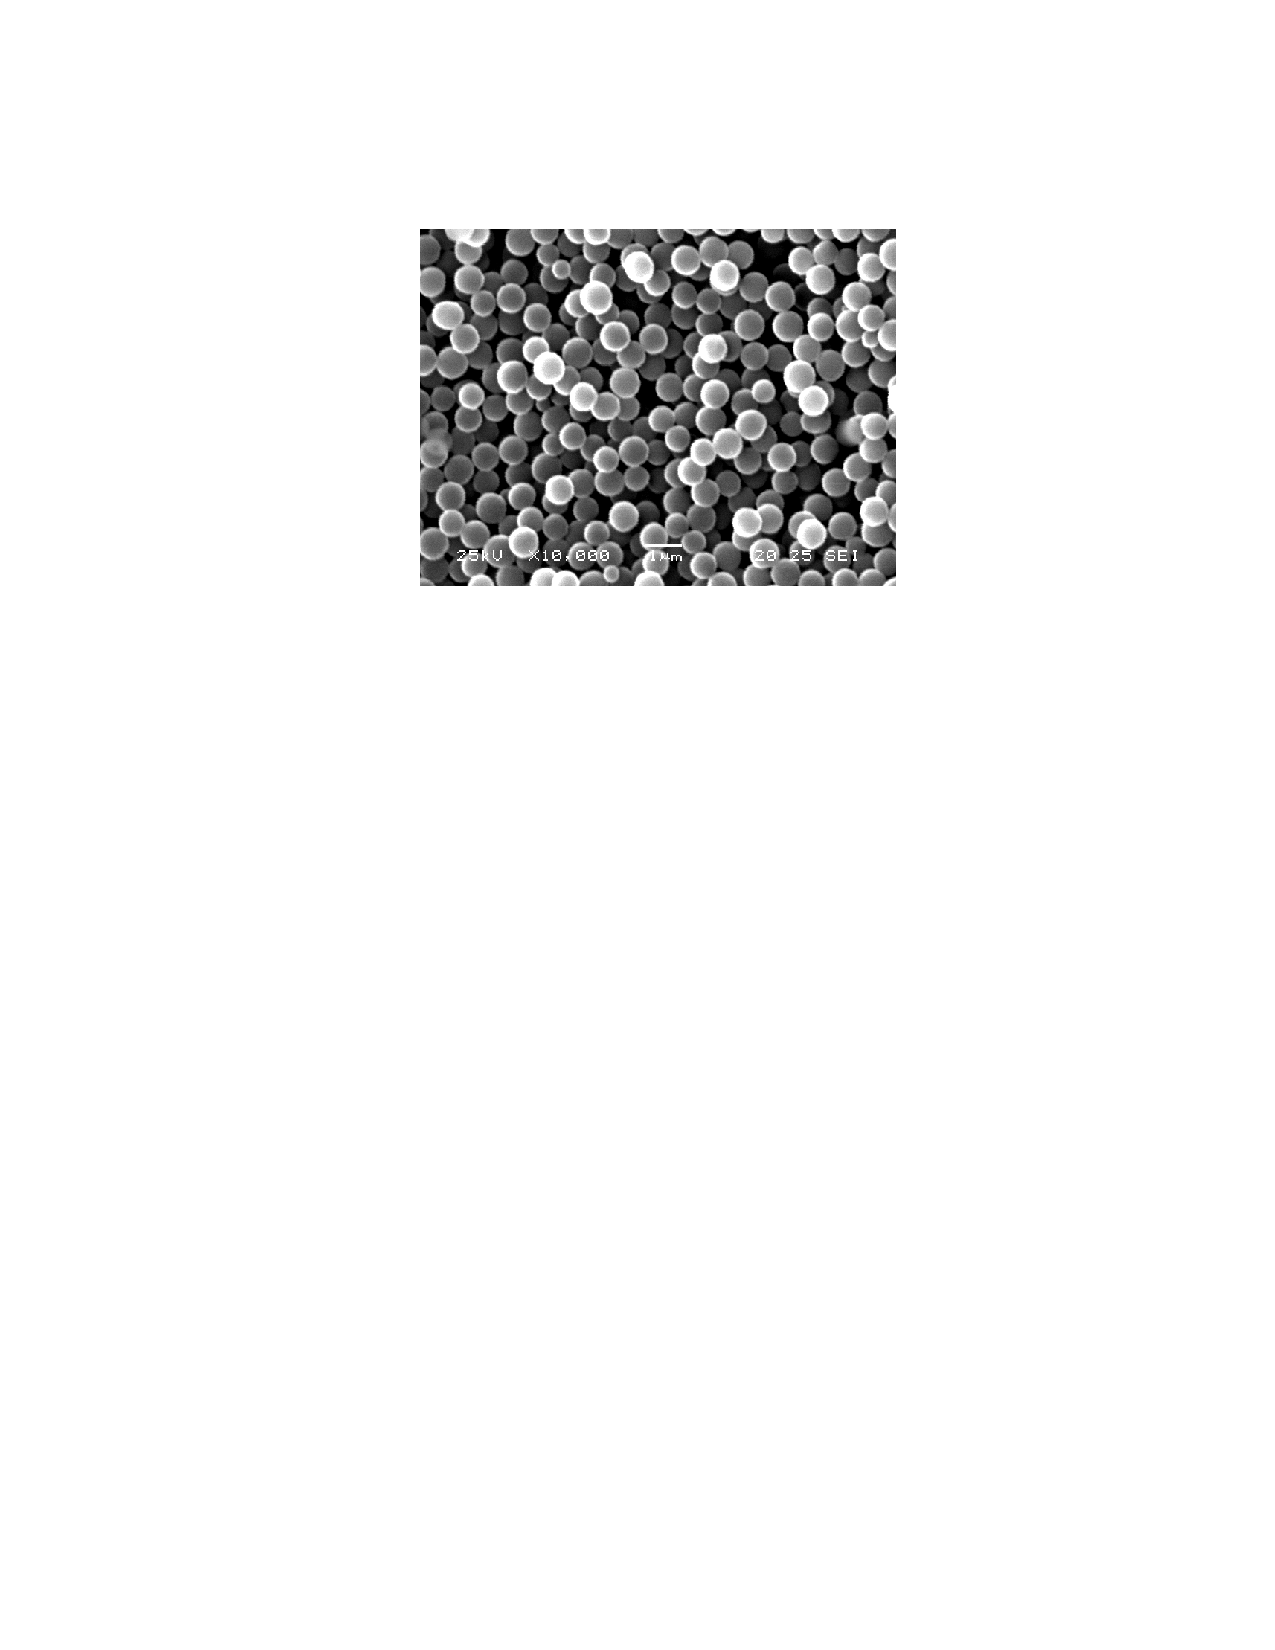
\includegraphics[width=\hsize]{Fernandez-Lahore/lahore_picture.pdf}
    \caption{sub-micrometer particles for bioseparation engineering}
     \end{center}
\end{figure}

%Achtung



\paragraph{Collaborations}
\begin{enumerate}
\item ChiPro GmbH - S.Bank - New bioprocess materials \item Pablo
Cassar\'{a} Laboratories Ltd (RA), M.A. Alvarez. \item Universidad
Nacional de Quilmes (RA) M. Grasselli.

\end{enumerate}


\nocite{Fernandez-Lahore1,Fernandez-Lahore2,Fernandez-Lahore3,Fernandez-Lahore4,Fernandez-Lahore5,Fernandez-Lahore6,Fernandez-Lahore7}
